\documentclass[11pt]{article}
\usepackage[a4paper, total={7in, 10in}]{geometry}
\usepackage{amsmath}
\usepackage{graphicx}
\usepackage{hyperref}
\graphicspath{ {./resources/} }
\usepackage[font=small,labelfont=bf]{caption} % Required for specifying captions to tables and figures
\usepackage[T1]{fontenc}
\usepackage[utf8]{inputenc}
\usepackage{listings}


\title{Scientific Computing - Systems of Equations}
\author{Mateusz Pełechaty}
\date{23 October 2022}%
\begin{document}
\maketitle

\section{Description}
Report showcases different methods of solving linear system of equations and their stability.
In other words we are going to solve the following problem for $\vec{x}$:
$$
    A \cdot \vec{x} = \vec{b}
$$
\begin{itemize}
    \item $A$ : specially defined, sparse matrix $n$ x $n$ of coefficients with parameter $l$ given on input
    \item $\vec{x}$ : vector of unknowns
    \item $\vec{b}$ : vector of constants
\end{itemize}
if we consider elements of $A$ as matrixes $l$ x $l$, then Matrix $A$ is a following tridiagonal matrix.
$$
    \begin{bmatrix}
        A_{1} & C_{1} & 0 & \dots & 0 & 0 \\
        B_{1} & A_{2} & C_{2} & \dots & 0 & 0 \\
        0 & B_{2} & A_{3} & \dots & 0 & 0 \\
        \vdots & \vdots & \vdots & \ddots & \vdots & \vdots \\
        0 & 0 & 0 & \dots & A_{n-1} & C_{n-1} \\
        0 & 0 & 0 & \dots & B_{n-1} & A_{n}
    \end{bmatrix}
$$
\begin{itemize}
    \item $A_{i}$ : dense matrix $l$ x $l$ of coefficients
    \item $B_{i}$ : matrix $l$ x $l$ of coefficients, where all elements are zeros except the first row and last column
    \item $C_{i}$ : matrix $l$ x $l$ of coefficients, where all elements are zeros except main diagonal
    \item 0: matrix $l$ x $l$ of zeros
\end{itemize}
Also $A$ is well conditioned matrix.
\section{Matrix data structure}
As we are going to use sparse matrices, we need to define a data structure for them, 
because it is inefficient to remember whole rows and columns.
I have decided to use a data structure following data structure to help me in the implementation of algorithms.
$$
    \begin{bmatrix}
        B_{0} & A_{1} & C_{1} & D_{1} \\
        B_{1} & A_{2} & C_{2} & D_{2} \\
        B_{2} & A_{3} & C_{3} & D_{3} \\
        \vdots & \vdots & \vdots & \vdots \\
        B_{n-2} & A_{n-1} & C_{n-1} & D_{n-1} \\
        B_{n-1} & A_{n-1} & C_{n} & D_{n}
    \end{bmatrix}
$$
where $D$ is matrix $l$ x $l$ on the right of matrix $C_i$ in $A$. \\
For constant $l$ we have $O(n)$ memory complexity.
\subsection*{Accessing to elements}
To access the elements of the matrix we need to define a function that will translate indexes of artificial matrix to indexes of real stored matrix.
As this is dependent on $l$ we need to pass it as a parameter.
\begin{lstlisting}
function indices(l, i, j)
    return i, l + j - l*div(i-1, l)
end
\end{lstlisting}
Translation of indexes if $O(1)$ and access to element of the matrix is $O(1)$.
Overall access to my data structure is $O(1)$

\section{Gaussian Elimination}
Gaussian elimination is a process, where we are trying to transform the matrix $A$ into an matrix, where all elements below the main diagonal are zeros.
Such matrix is called upper triangular matrix and it is easy to solve the system of equations with it.
\subsection*{Process Description}
We are trying going to consequently eliminate columns below the main diagonal starting from the first column.
So for every row below the main diagonal we are going to subtract row with the main diagonal element multiplied by a factor.
The factor is calculated as $\frac{A_{ij}}{A_{jj}}$ where $A_{ij}$ is the element below the main diagonal and $A_{jj}$ is the element on the main diagonal.
\subsection*{Acquiring solution}
After we have transformed the matrix $A$ into an upper triangular matrix, we can easily acquire the solution.
We can start from the last row and calculate the value of the last unknown.
Then we can use the value of the last unknown to calculate the value of the second to last unknown and so on.
It can be easily optimised, because acquired upper triangular matrix is of the special form best descripted on Figure $1$.
\begin{figure}[h]
    \centering
    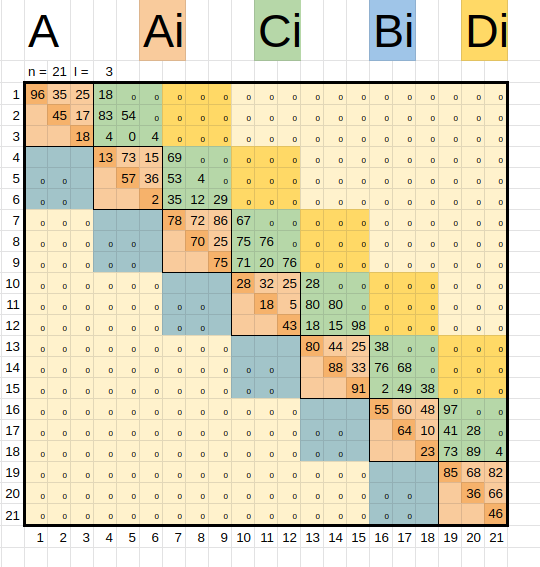
\includegraphics[width=0.6\textwidth]{gauss_solution.png}
    \caption{Upper triangular matrix after gaussian elimination}
\end{figure}
So we only need to update value of l rows after calculating the value of unknown
\subsection*{Code and Complexity} 
First let's look at function that zeroes cell below the main diagonal.
It calculates factor to multiply main diagonal row and substracts it from the row below the main diagonal.
\begin{lstlisting}
function zero_cell(matrix, l, b, row, diag_i)
    d = matrix[row, diag_i] / matrix[diag_i, diag_i]
    update b
    substract main diagonal * d from row below the main diagonal # O(l)
end
\end{lstlisting}
We can optimize substraction to only access $l$ elements, so it's time complexity is $O(l \cdot \alpha)$, where $\alpha$ is the complexity of accessing to matrix.
\newline
Now let's look at the function that performs Gaussian elimination.
We optimize the algorithm by performing only necessary operations. 
For the all diagonal elements except the last one in every matrix block we are going to remove elements below the main diagonal up to the next matrix block.
For the last diagonal element in every matrix block we are going to remove elements below the main diagonal up to the next matrix block.
\begin{lstlisting}
function gauss(matrix, b, n, l)
    for every matrix block  # O(n/l)
        for every main diagonal element except the last one # O(l)
            for every row below it until there are still zeroes # O(l) times
                zero_cell(matrix, l, b, row, diag_i) 
            end
        end

        diag_i = matrix_row + l
        for row from diag_i+1 to the next matrix block # O(l)
            zero_cell(matrix, l, b, row, diag_i) 
        end
    end
    return matrix, b
end
\end{lstlisting}
So the time complexity of the algorithm is 
$$O(n/l \cdot ( l \cdot l \cdot l \cdot \alpha + l \cdot l \cdot \alpha )) = O(n \cdot l^2 \cdot \alpha )$$
Considering my implementation, $\alpha$ is $O(1)$.
If $l$ is assumed constant then the time complexity is $O(n)$. We can further see it on Figure $2$
\begin{figure}[h]
    \centering
    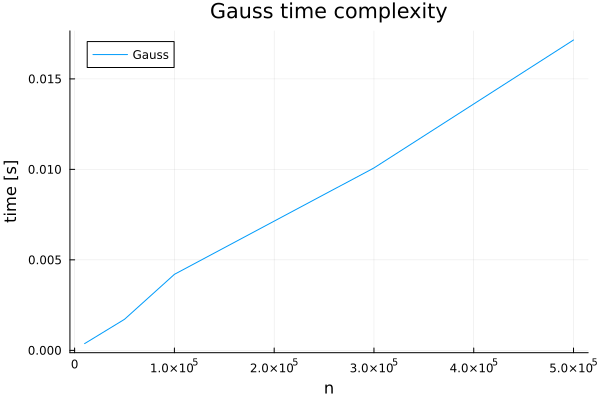
\includegraphics[width=0.6\textwidth]{gauss_time_complexity.png}
    \caption{Time complexity of Gaussian elimination}
\end{figure}
Additional Memory allocated by function is $O(1)$, as we are only creating temporary variables like iterators.
Total memory used by a function is $O(n)$, as we as this is the cost od $b$ and data structure containing matrix
\\
We can also look on the time and memory complexity of acquiring solution
\begin{lstlisting}
function get_solution_from_triangle_gauss(matrix, b, n, l)
    for i from n to 1 # O(n)
        b[i] /= matrix[i, i]     
        update b for all rows that contain non-zero i-th column # O(l)
    end
    return b
end
\end{lstlisting}
Note that we are not using additional memory to store x, as we are performing operations on b. 
\subsection*{Stability}
Relative error acquired from testing on matrices given as input is shown on Table $1$.
\begin{table}[!ht]
    \centering
    \begin{tabular}{|l|l|l|l|l|l|}
    \hline
        $n$ & 10000 & 50000 & 100000 & 300000 & 500000 \\ \hline
        error & 2.581075e-14 & 6.061823-14 & 7.3552517e-13 & 6.494568e-14 & 8.640995-14 \\ \hline
    \end{tabular}
    \caption{Relative errors of gauss elimination}
\end{table}
\\
As we can see, relative error of the algorithm does not depend on the size of the matrix if the matrix is well conditioned.
\\We can also look on how the error depends on the condition of the matrix.
Following tests were performed on matrices with n=20000, l=4. For every condition number we get average of 10 tests.
\begin{figure}[h]
    \centering
    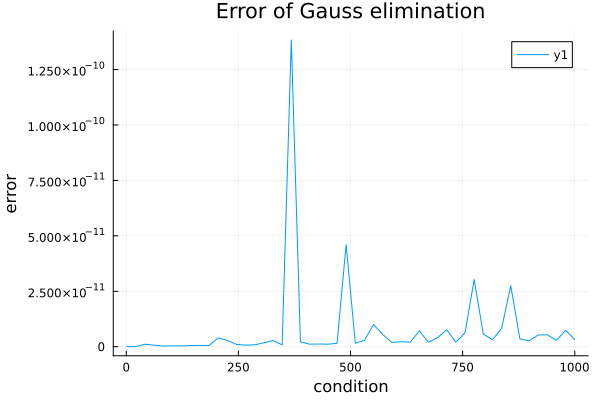
\includegraphics[width=0.6\textwidth]{gauss_error.png}
    \caption{Stability Experiment for gauss elimination}
\end{figure}
From the following we see that even though we took average, we can get matrix with relatively small condition number, but with high relative error.

\section{Gaussian Elimination with Partial Pivoting}
Gaussian elimination with partial pivoting is upgrade to normal Gaussian elimination in terms of stability.
It is done by swapping rows in order to get the biggest element on the main diagonal.

\subsection*{Process Description}
Process is almost the same as in Gaussian elimination, but before eliminating column below main diagonal,
we are going to swap rows in order to get the biggest element on the main diagonal.
\subsection*{Acquiring solution}
Acquiring solution is almost the same as in Gaussian elimination. 
The only difference is that we need to extend updating $b$ up to the next matrix block. So up to matrix $D_i$
\subsection*{Implementation and analysis} 
Code is almost the same as in Gaussian elimination, except for the fact that we need to swap rows and increase range of substracting rows up to $D_i$.
For that I will only show code for swapping rows.
\begin{lstlisting}
max_num_in_column, max_row = 0, 0 
for row below the main diagonal until nonzero # O(l)
    temp = abs(matrix[row, diag_i])
    if temp > max_num_in_column
        max_num_in_column = temp
        max_row = row
    end
end
swap_rows(matrix, l, diag_i, max_row)
swap(b, max_row, diag_i)
\end{lstlisting}
Swapping rows is $O(l)$, because non-zero elements will only appear in matrixes $A_i$, $B_i$, $C_i$ and $D_i$.
So the time complexity of the algorithm doesn't change because finding the biggest element and swap in column is $O(l)$ = $O(1)$.

Time complexity of acquiring solution also does not change, because we are only extending range of updating $b$ up to $D_i$. 
If $l$ is assumed constant then the time complexity is still $O(n)$. We can further see it on Figure $3$
\begin{figure}[h]
    \centering
    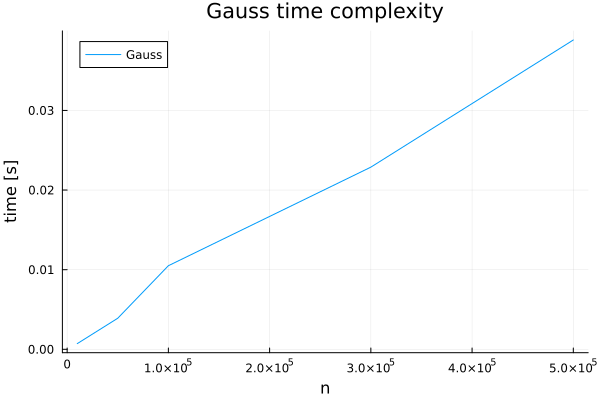
\includegraphics[width=0.6\textwidth]{gauss_choice_time_complexity.png}
    \caption{Time complexity of Gaussian elimination with partial pivoting}
\end{figure}
As we added only $O(1)$ memory operations, like finding maximum and swapping elements, thus additional memory usage is still $O(1)$.
\subsection*{Stability}
Relative error acquired from testing on matrices given as input is shown on Table $2$.
\begin{table}[!ht]
    \centering
    \begin{tabular}{|l|l|l|l|l|l|}
    \hline
        n & 10000 & 50000 & 100000 & 300000 & 500000 \\ \hline
        error & 4.91088e-16 & 5.33593e-16 & 5.12420e-16 & 4.49623e-16 & 4.44587-16 \\ \hline
    \end{tabular}
    \caption{Relative errors of Gauss elimination with partial pivoting}
\end{table}
As we can see, relative error of the algorithm does not depend on the size of the matrix if the matrix is well conditioned. 
We can also confirm that relative error is smaller than in Gaussian elimination without partial pivoting.
\\We can also look on how the error depends on the condition of the matrix.
Following tests were performed on matrices with n=20000, l=4. For every condition number we get average of 10 tests.
\begin{figure}[h]
    \centering
    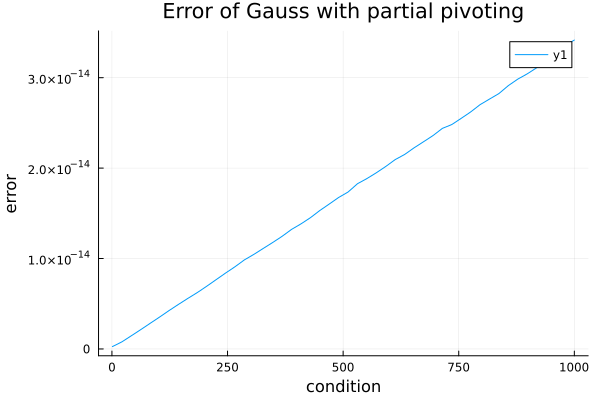
\includegraphics[width=0.6\textwidth]{gauss_pivot_error.png}
    \caption{Stability Experiment for gauss elimination}
\end{figure}
From the following we can see that partial pivoting makes the error(solution) stable and follow linear trend.
\section{LU Decomposition}
LU decomposition is a factorization of a matrix into a product of a lower and an upper triangular matrix.
By this we transform problem into
Lower triangular matrix consists of factors calculated during creation of upper triangular matrix when doing gaussian elimination.
By this we transform problem into 
$$Ax = b \rightarrow LU x = b$$
which we can further solve By solving $L \cdot y = b$ and $U \cdot x = y$.
\subsection*{Process Description}
Process is almost the same as in Gaussian elimination, but we are going to store factors in data structure described in section $2$.
And we are not going to update $b$ during substracting rows.
\subsection*{Acquiring solution}
To acquire solution from LU decomposition we need to solve $L \cdot y = b$ and $U \cdot x = y$. 
As the second one is solving upper triangular matrix, we can use the same algorithm as in Gaussian elimination.
For the lower one, we can modify the algorithm from Gaussian elimination to solve lower triangular matrix. We need to start from upper row and go down.
\subsection*{Implementation and analysis}
We are going to store L and U in the same data structure, so to not use any additional memory.
The only difference between this and Gaussian elimination is zero\_cell function so I will only show it.
\begin{lstlisting}
function zero_cell(matrix, l, b, row, diag_i)
    d = matrix[row, diag_i] / matrix[diag_i, diag_i]
    matrix[row, diag_i] = d
    substract main diagonal * d from row below the main diagonal # O(l)
    # consider only columns on the right of the main diagonal
end
\end{lstlisting}

As to solving equations with lower triangular matrix and upper we are going to use following function
\begin{lstlisting}
function get_solution_from_lu(matrix, b, n, l)
    for i in 1:n  # y calculation
        for down from i+1 to min(i+l,n)
            b[down] -= matrix[down, i]*b[i]
        end
    end # end y calculation
    return get_solution_from_triangle_gauss(matrix, b, n, l)
end
\end{lstlisting}
Note that loop that calculates y uses b as variable to store solution so we are not using any additional memory.
Function used to calculate x from y is the same as in Gaussian elimination.
In the end time complexity is still $O(n)$ and additional memory complexity is $O(1)$. We can confirm time complexity by looking at Figure $4$.
\begin{figure}[h]
    \centering
    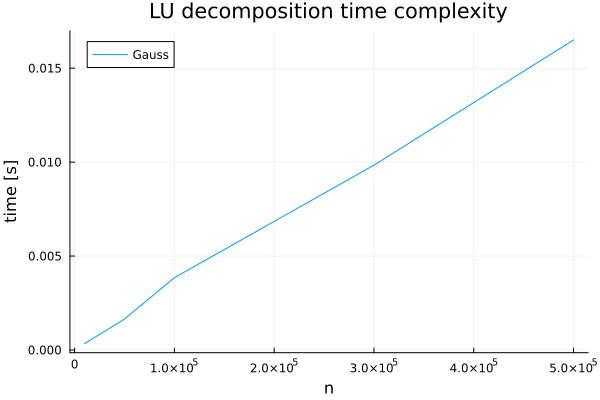
\includegraphics[width=0.6\textwidth]{lu_time_complexity.png}
    \caption{Time complexity of LU Decomposition}
\end{figure}
\subsection*{Stability}
Relative error acquired from testing on matrices given as input is shown on Table $3$.
\begin{table}[!ht]
    \centering
    \begin{tabular}{|l|l|l|l|l|l|}
    \hline
        n & 10000 & 50000 & 100000 & 300000 & 500000 \\ \hline
        error & 2.58107e-14 & 6.06182e-14 & 7.35525e-13 & 6.49456e-14 & 8.64099e-14 \\ \hline
    \end{tabular}
    \caption{Relative errors of LU decomposition} 
\end{table}
\\We can also look on how the error depends on the condition of the matrix.
Following tests were performed on matrices with n=20000, l=4. For every condition number we get average of 10 tests.
\begin{figure}[h]
    \centering
    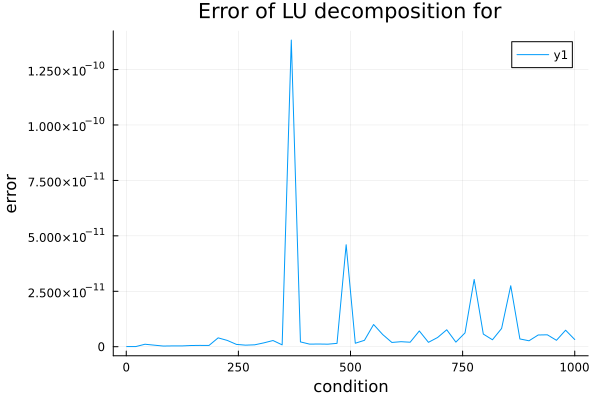
\includegraphics[width=0.6\textwidth]{lu_error.png}
    \caption{Stability Experiment for LU Decomposition}
\end{figure}
From this we can see that as stable as Gaussian elimination without partial pivoting.
\end{document} 